\documentclass[11pt,a4paper]{article}
\usepackage[T1]{fontenc}
\usepackage[utf8]{inputenc}
\usepackage{lmodern}
\usepackage[margin=25mm]{geometry}
\usepackage{amsmath,amssymb}
\usepackage{graphicx,booktabs,tabularx,array,float,placeins}
\usepackage{microtype}
\usepackage[font=small,labelfont=bf]{caption}
\usepackage[hidelinks]{hyperref}
\usepackage{xurl}
\graphicspath{{figures/}}
\setlength{\parindent}{1.2em}
\setlength{\parskip}{3pt}
\setlength{\emergencystretch}{2em}
\newcommand{\cancelterm}[1]{\underbrace{#1}_{\text{equal terms}}}
\hypersetup{pdftitle={AI651 Assignment 3: Traffic Forecasting on Graphs},pdfauthor={Muhammad Sami Ul Basit}}
\title{\textbf{Traffic Forecasting on Graphs}\\[4pt]\large AI651: Deep Learning for Space, Time and Graphs\\Assignment 3, Fall 2026}
\author{Muhammad Sami Ul Basit\\Roll No. 25280025\\Lahore University of Management Sciences}
\date{22 November 2026}
\begin{document}
\maketitle
\begin{center}\small Public repository: \url{https://github.com/msbasit/AI651_PA3}\end{center}

\begin{abstract}Questions 1-2 establish what aggregation preserves and how direction can enter a graph layer. Questions 3-7 implement four lightweight forecasters using all 716 San Diego sensors, 2020 training data, January-March 2021 validation data, and April-December 2021 test data. Each prediction uses eight 15-minute observations and forecasts four further intervals.

The lowest measured test MAE is from \textbf{adaptive}: \textbf{52.72} vehicles per 15 minutes. This is a 14.63\% relative MAE reduction versus temporal-only. These are single-seed, finite-budget comparisons; they do not establish a universal ranking or statistical significance.\end{abstract}

\begin{table}[H]
\centering\small
\caption{Final test comparison in vehicles per 15-minute interval.}
\renewcommand{\arraystretch}{1.16}
\begin{tabularx}{\linewidth}{@{}>{\raggedright\arraybackslash}X>{\raggedright\arraybackslash}X>{\raggedright\arraybackslash}X>{\raggedright\arraybackslash}X>{\raggedright\arraybackslash}X@{}}
\toprule
\textbf{Model} & \textbf{Adjacency} & \textbf{MAE} & \textbf{RMSE} & \textbf{Train time (s)} \\
\midrule
Temporal-only & None & 61.75 & 97.28 & 780.0 \\
STGNN & Fixed & 58.88 & 92.48 & 930.9 \\
STGNN & Adaptive & 52.72 & 83.58 & 970.8 \\
STGNN & Hybrid & 55.11 & 87.19 & 609.7 \\
Persistence & None & 87.11 & 132.88 & 0 (untrained) \\
\bottomrule
\end{tabularx}
\end{table}


{\small Persistence repeats the last observed value at each sensor for all four horizons. On the same test masks it scores MAE 87.11 and RMSE 132.88. Averaging last values in original units through the revised fixed graph with one unit self-loop instead scores MAE 170.97 and RMSE 247.55; this is an aggregation diagnostic, not a learned model. The graph models retain a separate local path.}


{\small Errors are in vehicles per 15-minute interval. Metrics pool every valid sensor/horizon target over the same full test period. Training times include all executed epochs and epoch validation, with synchronized XPU wall time; preparation, warmup and final evaluation are excluded. Early stopping can give different realized durations under the same rule.}


{\small Timing precision: every displayed total is independently rounded from its own synchronized run. Unrounded seconds, actual epoch counts and individual epoch durations are retained in metrics.json and the per-model history files; equality after rounding does not imply shared timing measurements.}


Intel(R) Core(TM) Ultra 7 255H; 46.9 GiB system RAM. Training and primary inference: Intel(R) Arc(TM) 140T GPU (23GB) using PyTorch 2.14.1+xpu. Additional full-test inference: Intel AI Boost through OpenVINO 2026.4.1. The GPU memory label describes shared integrated-GPU memory, not dedicated VRAM.


\FloatBarrier\section{What does a sum remember?}\label{sec:q1}
\subsection{Affine messages retain only degree and total trend}

Let \(n_v=|\mathcal N(v)|\) and \(S_v=\sum_{u\in\mathcal N(v)}x_u\). For scalar or vector parameters \(w,c\),
\begin{equation}\label{eq:affine}
\sum_{u\in\mathcal N(v)}\phi(x_u)
=\sum_{u\in\mathcal N(v)}(wx_u+c)=wS_v+cn_v.
\end{equation}
Equal \(n_v\) and \(S_v\) therefore force the same aggregate for every \(w,c\); applying any function \(\rho\) preserves this equality. For example, the neighborhoods \(\{-1,+1\}\) and \(\{0,0\}\) both have \(n_v=2\) and \(S_v=0\), but contain zero and two steady neighbors, respectively.


\subsection{A single nonlinear scalar can encode all three counts}

Choose base \(B=K+1\) and assign
\begin{equation}
\phi(-1)=1,\qquad \phi(0)=B,\qquad \phi(+1)=B^2.
\end{equation}
If the three counts are \((n_-,n_0,n_+)\), their aggregate is
\begin{equation}q=n_-+Bn_0+B^2n_+.\end{equation}
Each count is at most \(K<B\), so no carries occur. The counts are the base-\(B\) digits:
\begin{align}
n_-&=q\bmod B, & n_0&=\left\lfloor\frac qB\right\rfloor\bmod B,
& n_+&=\left\lfloor\frac q{B^2}\right\rfloor\bmod B.
\end{align}


For \(K=8\), the base is \(B=9\). Exhaustive NumPy enumeration checks
\begin{equation}\binom{K+3}{3}-1=\binom{11}{3}-1=164\end{equation}
nonempty count triples with total at most eight. Every code is distinct and every triple decodes exactly. To count only non-steady neighbors at any degree, choose
\begin{equation}\phi(x)=x^2\quad\Longrightarrow\quad\sum_{u\in\mathcal N(v)}\phi(x_u)=n_-+n_+.\end{equation}


\subsection{Fixed one-hot messages: complete comparison}

Write the count vector as \((s,z,p)\), with \(n=s+z+p\). Coordinates refer to slowing, steady and speeding up, respectively. All counterexamples below satisfy \(1\le n\le8\).


\begin{table}[H]
\centering\small
\caption{Information retained by one-hot sum, mean and max aggregation.}
\renewcommand{\arraystretch}{1.16}
\begin{tabularx}{\linewidth}{@{}>{\raggedright\arraybackslash}p{.16\linewidth}>{\raggedright\arraybackslash}p{.10\linewidth}>{\raggedright\arraybackslash}p{.11\linewidth}>{\raggedright\arraybackslash}X@{}}
\toprule
\textbf{Task} & \textbf{Method} & \textbf{Possible?} & \textbf{Explicit calculation or indistinguishable pair} \\
\midrule
Count steady & Sum & Yes & \(\rho(s,z,p)=z\). \\
Count steady & Mean & No & \{0\} and \{0,0\} both aggregate to (0,1,0), but their correct counts are 1 and 2. \\
Count steady & Max & No & \{0\} and \{0,0\} both aggregate to (0,1,0), but their correct counts are 1 and 2. \\
Slowing majority & Sum & Yes & Test \(2s>s+z+p\). \\
Slowing majority & Mean & Yes & Test \(s/n>\tfrac12\). \\
Slowing majority & Max & No & \{-1,-1,+1\} and \{-1,+1,+1\} both aggregate to (1,0,1); correct answers are True and False. \\
Any slowing & Sum & Yes & Test \(s>0\). \\
Any slowing & Mean & Yes & Test \(s/n>0\), since \(n>0\). \\
Any slowing & Max & Yes & Test whether the first coordinate equals \(1\). \\
\bottomrule
\end{tabularx}
\end{table}


\FloatBarrier\section{Which way is the slowdown moving?}\label{sec:q2}
\subsection{Equal weights diffuse the pattern}

For an impulse at sensor 20, the predictions at sensors \((19,20,21)\) are \((b,a,b)\), while the targets are \((1,0,0)\). All other predictions and targets vanish. Hence
\begin{align}
\mathcal L(a,b)&=(b-1)^2+a^2+b^2,\\
\frac{\partial\mathcal L}{\partial a}&=2a=0,
&\frac{\partial\mathcal L}{\partial b}&=4b-2=0.
\end{align}
The unique minimizer is \(a=0\), \(b=\tfrac12\), with \(\mathcal L_{\min}=\tfrac12\). Its Hessian \(\operatorname{diag}(2,4)\) is positive definite.


\begin{figure}[H]\centering
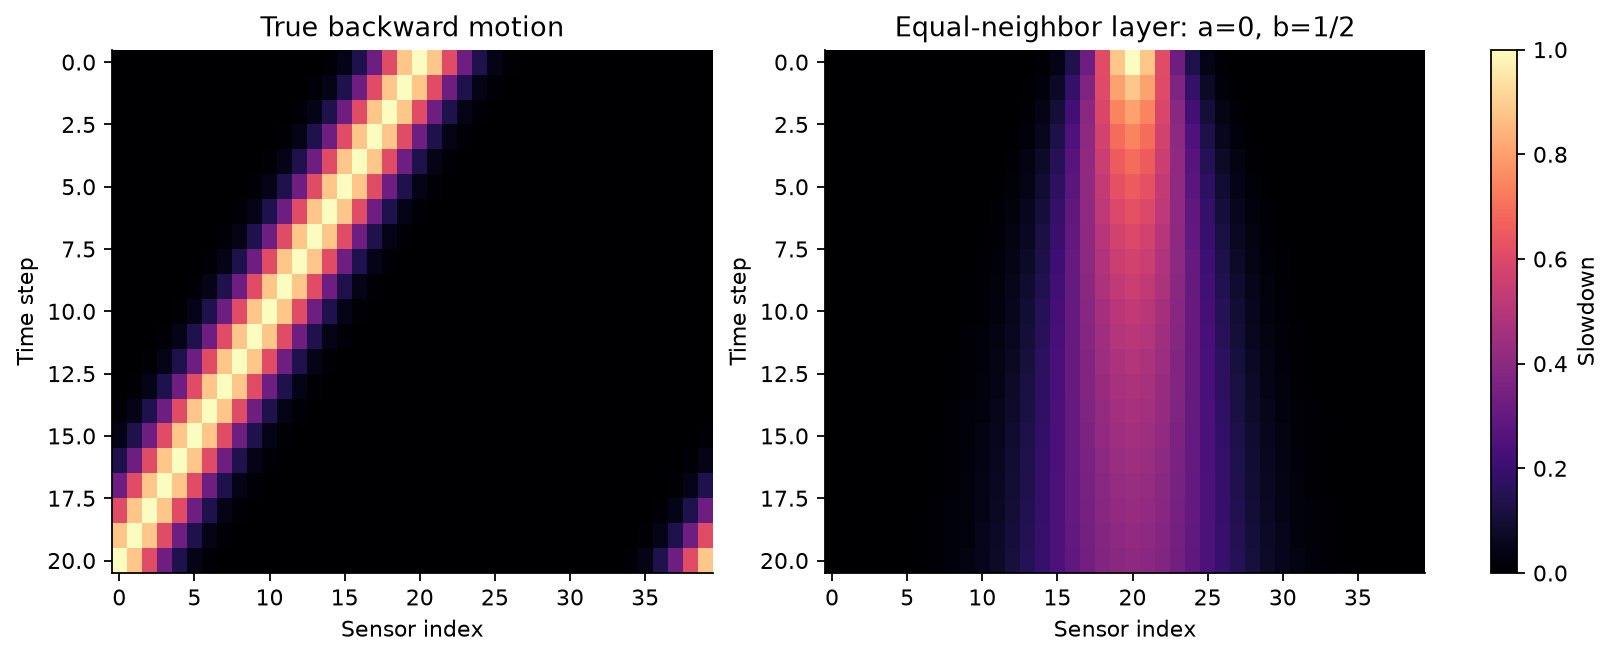
\includegraphics[width=\linewidth,height=.34\textheight,keepaspectratio]{q2_rollouts.png}
\caption{Both sequences start from \(\exp(-(i-20)^2/8)\), use the same [0,1] color scale and show t=0,...,20. The fitted symmetric rule is applied recursively without teacher forcing.}
\end{figure}

The true bump moves one sensor against traffic at every step and preserves its height and shape; periodic wrapping is visible in the true-motion panel near the ring boundary. The equal-neighbor layer spreads mass both ways, lowering and widening the peak rather than translating it.


\subsection{Give the layer direction labels}

Choose
\begin{equation}a=0,\qquad w_-=0,\qquad w_+=1.\end{equation}
Then \(\widehat x_i(t+1)=x_{i+1}(t)\), exactly the required motion for every input. A PyTorch \texttt{Conv1d} cross-correlation uses
\begin{equation}\underbrace{[\,0,\ 0,\ 1\,]}_{\text{kernel}}\quad\text{on}\quad[x_{i-1},x_i,x_{i+1}],\end{equation}
with circular padding of one and no bias. A mathematical convolution reverses its stored-kernel convention. In part (a), sensors 19 and 21 are forced to receive the same prediction \(b\), so the asymmetric target \((1,0)\) cannot be fitted. Separate \(w_-\) and \(w_+\) remove this constraint. Direction labels therefore break the reflection ambiguity that persists through stacks of unlabeled symmetric layers.


\subsection{History supplies the missing directional information}

Choose \(a=0\), \(b=1\), \(c=-1\), so that
\begin{equation}\widehat x_i(t+1)=x_{i-1}(t)+x_{i+1}(t)-x_i(t-1).\end{equation}
For backward motion, \(x_{i-1}(t)=x_i(t-1)\); substitution gives
\begin{equation}\widehat x_i(t+1)=\cancelterm{x_{i-1}(t)}+x_{i+1}(t)-\cancelterm{x_i(t-1)}=x_{i+1}(t).\end{equation}
For forward motion, \(x_{i+1}(t)=x_i(t-1)\), so the same coefficients give
\begin{equation}\widehat x_i(t+1)=x_{i-1}(t)+\cancelterm{x_{i+1}(t)}-\cancelterm{x_i(t-1)}=x_{i-1}(t).\end{equation}
Since \(x_{i-1}(t)\) is exactly the forward-motion target, the same coefficients \((a,b,c)=(0,1,-1)\) still work.


The past local value identifies the spatial term associated with where the pattern has already passed. Subtracting it leaves the opposite neighbor, even though both spatial coefficients remain equal. This exact identity assumes the stated constant-speed, shape-preserving motion; noise or changing speed need not satisfy it. Numerical checks verify both directions to floating-point precision.


\FloatBarrier\section{Dataset preparation and graph construction}\label{sec:q3}\subsection{Data extraction and resampling}
\subsubsection{Source, sensor identity and units}

The official LargeST repository \cite{largest-repo} specifies District 11 for SD and maps sensor IDs to adjacency indices using metadata ID2. Kaggle API requests returned empty HTTP 404 responses on this machine. Raw 2020/2021 HDF5 files, metadata and adjacency were therefore obtained from a public mirror \cite{mirror}. Downloads use a pinned mirror revision and verify LFS SHA-256 digests. These checks establish transfer integrity against the mirror; equivalence to an independently downloaded Kaggle archive was not verified.


All 8,600 HDF column IDs are checked against the complete metadata order. The 716 District-11 rows then select both the traffic columns by ID and the graph by ID2. The raw five-minute grid is reindexed to the full calendar year, preserving missing timestamps explicitly.


PeMS defines five-minute total flow in vehicles per five minutes~\cite{pems}. We therefore preserve interval volume by summing:
\begin{equation}\label{eq:resample}
X^{(15\,\mathrm{min})}_t=\sum_{k=0}^{2}X^{(5\,\mathrm{min})}_{3t+k}.
\end{equation}
The resulting unit is vehicles per 15-minute interval. This follows the assignment's count-volume option. The official benchmark notebook averages and rounds~\cite{largest-repo}; our errors consequently use a different physical scale and should not be compared directly with that benchmark's reported values.


\subsubsection{Missing values and split-local preprocessing}

Nonfinite or negative five-minute values are invalid: 3,095,400 in 2020 and 4,541,266 in 2021. A 15-minute target is valid only if all three inputs are valid (sum with min\_count=3). Zeros remain valid; no observation-quality flags are available to distinguish genuine zero flow from undocumented outage zeros.


\begin{table}[H]
\centering\small
\caption{Chronological splits and valid-label availability.}
\renewcommand{\arraystretch}{1.16}
\begin{tabularx}{\linewidth}{@{}>{\raggedright\arraybackslash}X>{\raggedright\arraybackslash}X>{\raggedright\arraybackslash}X>{\raggedright\arraybackslash}X@{}}
\toprule
\textbf{Split} & \textbf{15-min bins} & \textbf{Windows} & \textbf{Missing sensor-bins} \\
\midrule
2020 training & 35,136 & 35,125 & 1,034,655 \\
Jan-Mar 2021 validation & 8,640 & 8,629 & 376,574 \\
Apr-Dec 2021 testing & 26,400 & 26,389 & 1,139,060 \\
\bottomrule
\end{tabularx}
\end{table}


Within each split, input gaps are forward-filled, with each sensor's training median as the fallback at the beginning of a split (zero only if that sensor has no training observations). Validation/test values never enter training statistics. Missing targets are excluded from the loss and every reported error; filled targets are never treated as labels.


\begin{figure}[H]\centering
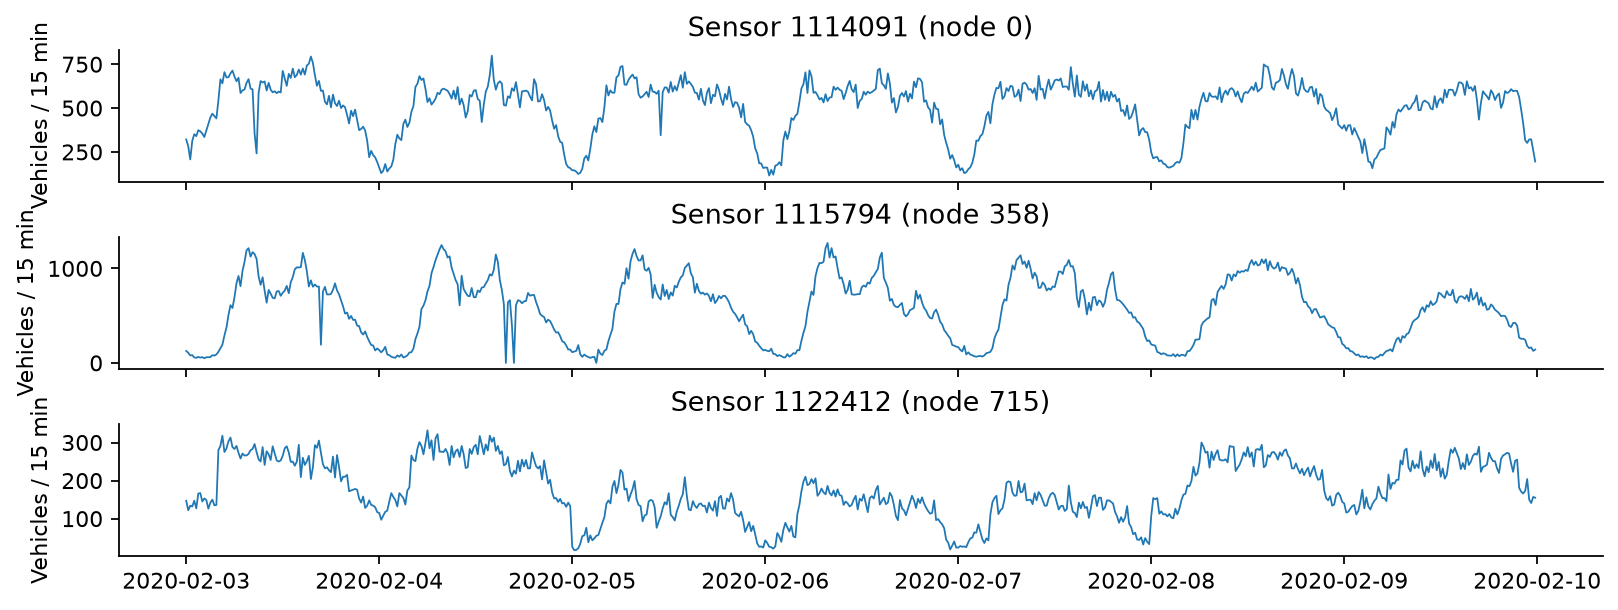
\includegraphics[width=\linewidth,height=.34\textheight,keepaspectratio]{q3_week.png}
\caption{Complete calendar week, 3-9 February 2020. Sensors are predetermined nodes 0,358,715; gaps remain visible in the observed series.}
\end{figure}

\FloatBarrier\subsection{Road graph and neighborhoods}
\subsubsection{Graph construction and direction}

The SD matrix is 716\ensuremath{\times}716. It contains \textbf{18,035} nonzero ordered entries including \textbf{716} diagonal entries, or \textbf{17,319} non-self directed entries. It is \textbf{not symmetric}; \(\max_{i,j}|A_{ij}-A_{ji}|=1.000000\). Non-self row degree ranges from 0 to 70, with mean 24.19. Ordered entries are reported rather than silently halving a directed edge count.


A nonzero \(A_{ij}\) is a retained road-distance weight. LargeST constructs strengths using a thresholded Gaussian of shortest driving distance~\cite{largest-paper}:
\begin{equation}
A_{ij}=\begin{cases}\exp(-d_{ij}^2/\sigma^2),&\exp(-d_{ij}^2/\sigma^2)\ge r,\\0,&\text{otherwise}.\end{cases}
\end{equation}
The entry is a strength, not the distance itself. In our multiplication convention, row \(i\) receives node \(j\)'s features with this weight; this does not necessarily mean that vehicles travel from \(j\) to \(i\).


\begin{figure}[H]\centering
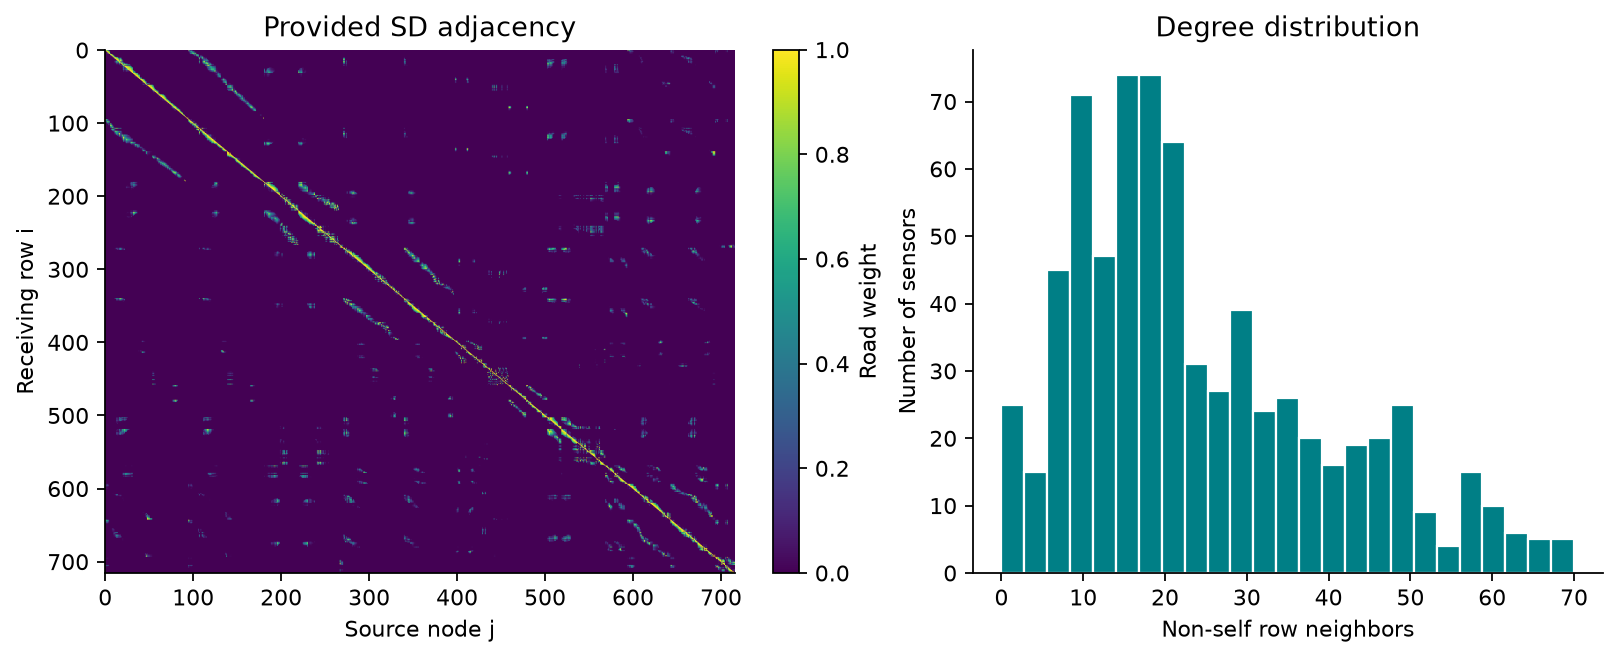
\includegraphics[width=\linewidth,height=.34\textheight,keepaspectratio]{q3_graph.png}
\caption{Adjacency in the verified sensor order and distribution of non-self row neighbors. Raw self-loops are included in the heatmap and excluded from the degree count.}
\end{figure}

\subsubsection{Example: sensor 1126411 (node 33)}

The example uses only the road graph: the first node whose non-self degree is closest to the median. The following lists implement the assignment's definition literally,
\begin{equation}\mathcal N(i)=\{j:A_{ij}\ne0\}.\end{equation}
A provided self-loop therefore includes the focal sensor itself; the degree histogram excludes self-loops.


\textbf{One-hop sensor IDs:} 1126411, 1114805, 1114035, 1108547, 1118707, 1117871, 1108615, 1117818, 1126426, 1114806, 1108711, 1108693, 1111514, 1113486, 1115356, 1115413, 1115432, 1115438, 1116574, 1115528, 1115517.


\textbf{At-most-two-hop sensor IDs:} 1117748, 1113976, 1117741, 1108603, 1117835, 1117717, 1118078, 1108611, 1108613, 1114050, 1108617, 1118496, 1126411, 1114805, 1114035, 1108547, 1118707, 1118521, 1108665, 1117683, 1108417, 1117734, 1108605, 1118702, 1108609, 1117871, 1108615, 1117818, 1126426, 1114806, 1108711, 1108693, 1111514, 1108728, 1114540, 1113486, 1115356, 1115413, 1115432, 1115438, 1111551, 1115420, 1115426, 1111566, 1115444, 1116783, 1114546, 1116574, 1115528, 1115517, 1115555, 1115565, 1111552, 1116165, 1115548, 1111540, 1115572, 1121818, 1114450, 1114457, 1113279, 1111539, 1108331, 1111520, 1121821, 1114463, 1111509, 1121288, 1116112, 1113460, 1108572, 1115921, 1108391, 1115929.


The focal sensor 1126411 is included in both literal lists because the supplied graph has a self-loop at that sensor. The non-self one-hop and two-hop lists are also saved separately in preparation.json.


Nearby sensors can reveal upstream congestion, downstream bottlenecks and common demand changes before the local series fully reflects them. One layer combines immediate row neighbors. Two layers can propagate information along paths of length two, while repeated self-loops also retain shorter paths. More layers can blend distinct local states (oversmoothing), compress many distant signals (oversquashing), increase noise and overfit; greater depth is therefore not automatically better.


\FloatBarrier\section{Spatio-temporal forecasting}\label{sec:q4}
\subsection{Forecast windows and normalization}

A split of length \(T\) supplies exactly \(T-11\) windows, indexed by \(s=0,\ldots,T-12\):
\begin{align}
X_s&=[x_s,x_{s+1},\ldots,x_{s+7}],\\
Y_s&=[x_{s+8},x_{s+9},x_{s+10},x_{s+11}].
\end{align}
Thus \(X_s\in\mathbb R^{8\times716\times1}\), \(Y_s\in\mathbb R^{4\times716\times1}\). Batched tensors add a leading dimension \(B\). No input or target crosses a split boundary; validation and test history also begins within its own split.


Per-sensor training statistics are computed from the filled 2020 series only. Each sensor is standardized with its own mean and standard deviation. Across sensors, means range from 0.00 to 1334.65, and used standard deviations range from 1.00 to 822.44. For 19 constant training sensors, a unit scale avoids division by zero. Every forecast is inverted with that sensor's statistics before scoring.
\begin{equation}\widetilde x_{t,i}=\frac{x_{t,i}-\mu_i}{\sigma_i},\qquad \widehat y_{s,h,i}=\sigma_i\widehat{\widetilde y}_{s,h,i}+\mu_i.\end{equation}


\subsection{Architecture and controlled baseline}

\begin{table}[H]
\centering\small
\caption{Shared forecasting architecture.}
\renewcommand{\arraystretch}{1.16}
\begin{tabularx}{\linewidth}{@{}>{\raggedright\arraybackslash}p{.21\linewidth}>{\raggedright\arraybackslash}X@{}}
\toprule
\textbf{Stage} & \textbf{Operation / shape} \\
\midrule
Temporal encoder & Two temporal convolutions, \(1\to16\) then \(16\to16\) channels, each with a \(1\times3\) kernel, \((0,1)\) padding and ReLU. Node positions are not mixed. \\
Temporal representation & Flatten each sensor\textquotesingle s \(16\times8\) feature map; apply \(\operatorname{Linear}(128,16)\), giving \(Z\in\mathbb R^{B\times716\times16}\). \\
Local and graph layer & \(H=\operatorname{ReLU}(ZW_{\mathrm{local}}+\widehat A ZW_g)\). Both \(16\times16\) projections have no bias. The local representation survives independently of graph averaging. \\
Forecast head & \(\operatorname{Linear}(16,4)\) per sensor, yielding \(\widehat Y\in\mathbb R^{B\times4\times716\times1}\). All horizons are predicted directly. \\
Temporal-only & Same temporal encoder, local projection and head, with \(H=\operatorname{ReLU}(ZW_{\mathrm{local}})\). No graph term. \\
\bottomrule
\end{tabularx}
\end{table}


Trainable parameters: temporal-only \textbf{3,236}, fixed \textbf{3,492}, and adaptive/hybrid \textbf{17,812}. The graph variants add a 16\ensuremath{\times}16 graph projection; adaptive/hybrid also add two 716\ensuremath{\times}10 embeddings. Shared encoder, local projection and head initial weights are identical across experiments.


\subsection{Training and model selection}

All runs use seed 25280025, FP32, Adam (lr 0.002, weight decay 0.0001 on forecasting weights and zero on graph embeddings), batch 64, norm clipping at 5, maximum 40 epochs and patience 5. Every training window is used, with identical epoch-seeded shuffles. Minimum full-validation MAE selects the checkpoint. The revision protocol was set from the independent review; test results are not used for further hyperparameter selection. Fixed seeds do not guarantee bitwise XPU determinism.


The loss is masked MAE after per-sensor inverse scaling, divided by one fixed training-only global flow scale for numerical conditioning. This preserves equal original-unit weighting across sensors rather than giving low-variance sensors greater loss weight. Filled labels are excluded and real zeros retained. Overlapping-window horizon forecasts count separately, with identical masks for all models. Final metrics use the validation-selected checkpoint.
\begin{equation}\mathcal L_{\mathcal B}=\frac{1}{s_{\mathrm{train}}C_{\mathcal B}}\sum_{(s,h,i)\in\mathcal B}m_{s,h,i}\,\sigma_i\left|\widehat{\widetilde y}_{s,h,i}-\widetilde y_{s,h,i}\right|.\end{equation}
Here \(C_{\mathcal B}\) counts valid batch targets, and \(s_{\mathrm{train}}\) is one scalar standard deviation of the filled training counts, shared by every model.


\begin{figure}[H]\centering
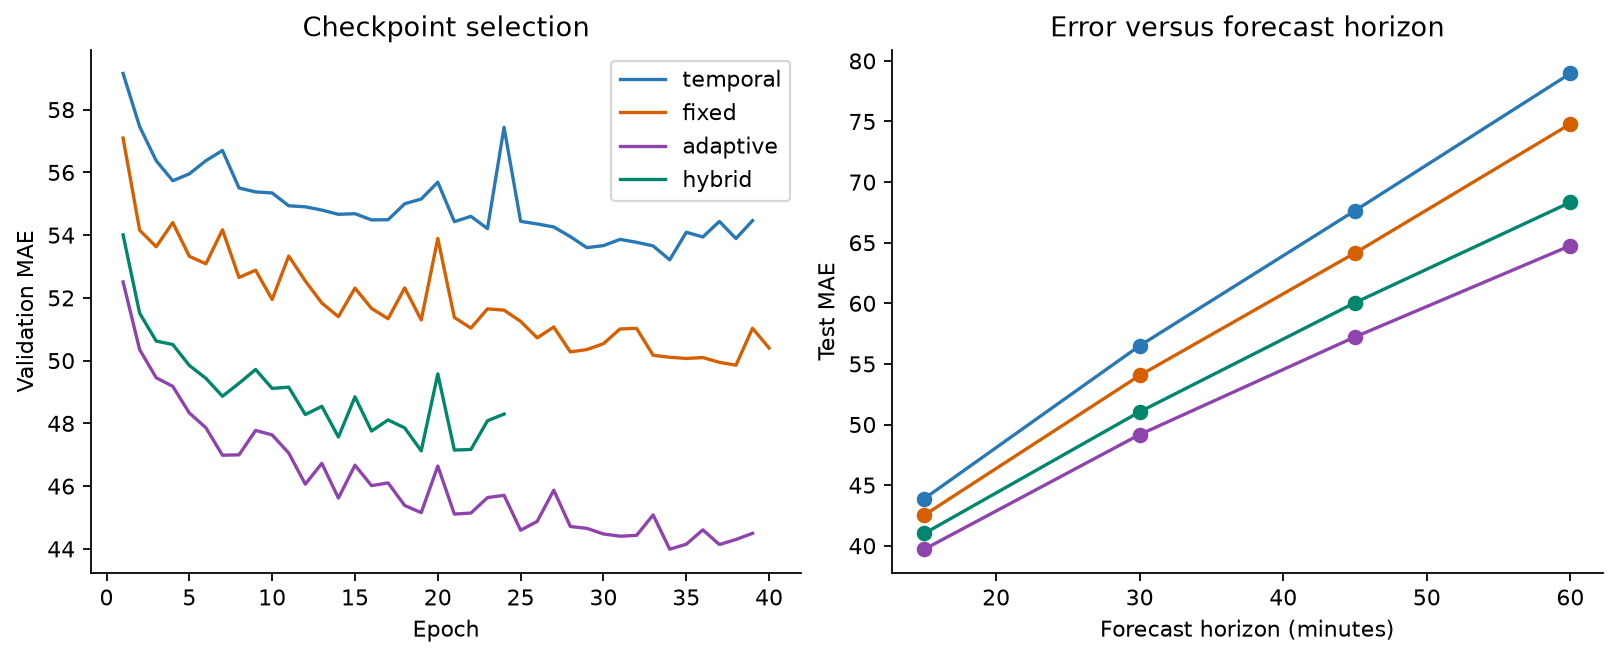
\includegraphics[width=\linewidth,height=.34\textheight,keepaspectratio]{q6_learning.png}
\caption{Validation learning curves and test MAE at 15,30,45,60 minutes. The latter uses each model's validation-selected checkpoint.}
\end{figure}

\FloatBarrier\section{Fixed, adaptive and hybrid adjacency}\label{sec:q5}
\subsection{Fixed graph}

The fixed graph uses directed row normalization:
\begin{equation}\label{eq:fixed}
\widehat A_{\mathrm{fixed}}=D^{-1}(A_{\mathrm{off}}+I),\qquad D_{ii}=\sum_j(A_{\mathrm{off}}+I)_{ij}.
\end{equation}
Here \(A_{\mathrm{off}}=A-\operatorname{diag}(\operatorname{diag}A)\). Clearing the supplied diagonal before adding \(I\) gives exactly one unit self-loop. Each receiving row is a nonnegative weighted average; directed normalization avoids assuming symmetry. The raw graph remains unchanged for Section~\ref{sec:q3}; the normalized model graph is a nontrainable buffer throughout optimization.


\subsection{Learnable graph}

Introduce two trainable matrices \(E_1,E_2\in\mathbb R^{716\times10}\), independently initialized from \(\mathcal N(0,1)\). Define
\begin{align}
L&=\operatorname{ReLU}(E_1E_2^{\mathsf T}),\\
(\widehat A_{\mathrm{adaptive}})_{ij}&=\frac{\exp L_{ij}}{\sum_{k=1}^{716}\exp L_{ik}}.
\end{align}
The standard-normal initialization produces nontrivial logits rather than an almost uniform initial graph. Gradients flow through row softmax, positive ReLU logits and the embedding product; negative logits have zero ReLU gradient on that step. All 716 neighbors are retained, with no top-\(k\) training sparsification.


\subsection{Hybrid graph}

Combine the consistently normalized matrices using
\begin{equation}\label{eq:hybrid}
\widehat A_{\mathrm{hybrid}}=\alpha\widehat A_{\mathrm{fixed}}+(1-\alpha)\widehat A_{\mathrm{adaptive}},\qquad\alpha=0.5.
\end{equation}
Both terms are row stochastic, so their convex combination remains normalized. The hybrid has its own learned embeddings under the same training protocol. The mixing coefficient is fixed, rather than selected using test performance.


\begin{figure}[H]\centering
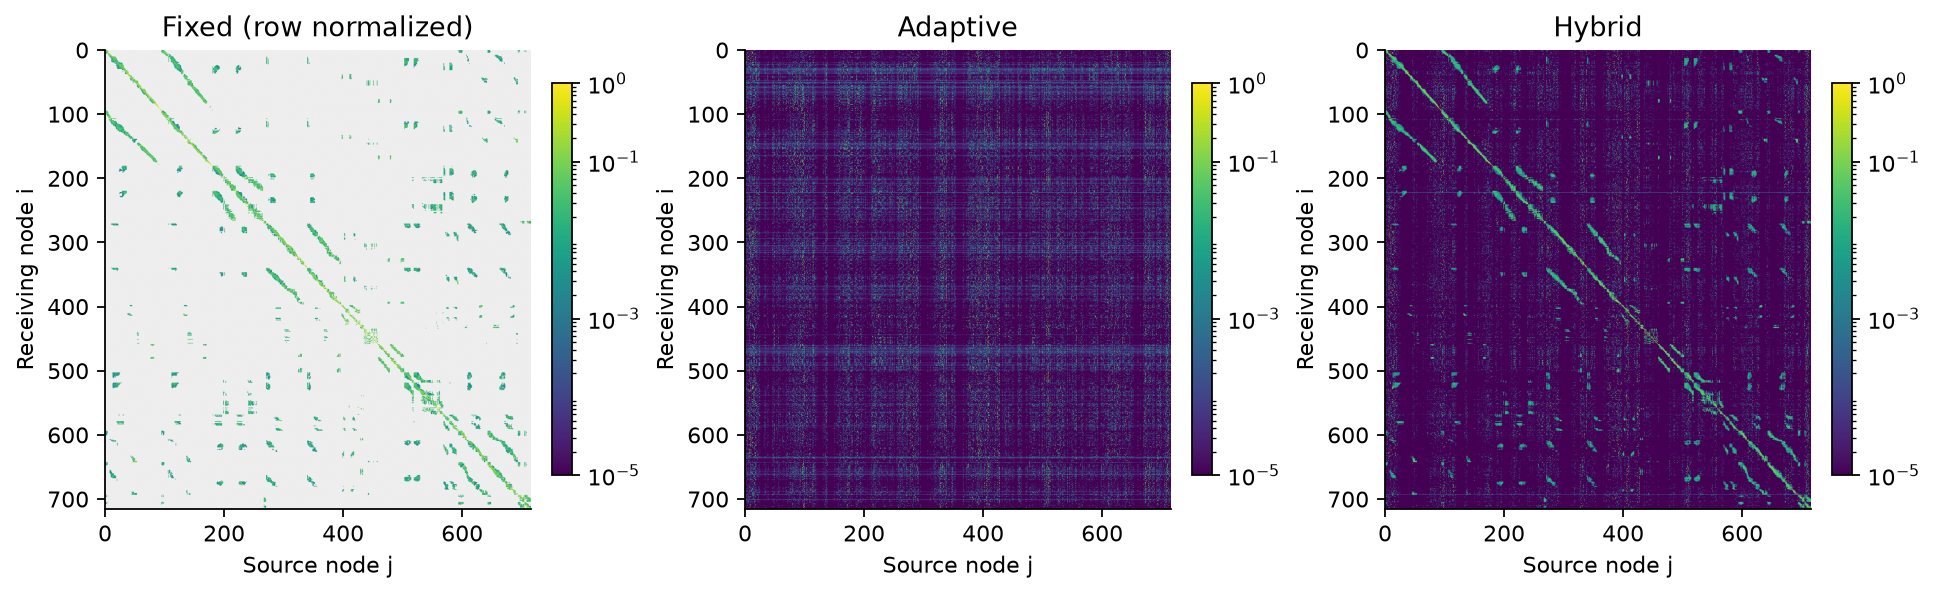
\includegraphics[width=\linewidth,height=.34\textheight,keepaspectratio]{q5_adjacencies.png}
\caption{Final node-mixing matrices for the validation-selected checkpoints. All panels share a logarithmic weight scale from 0.00001 to 1. Zero weights are gray; smaller positive weights use the lowest display color. This is display clipping only: no graph weights are pruned.}
\end{figure}

\begin{table}[H]
\centering\small
\caption{Validation and test errors for validation-selected checkpoints.}
\renewcommand{\arraystretch}{1.16}
\begin{tabularx}{\linewidth}{@{}>{\raggedright\arraybackslash}X>{\raggedright\arraybackslash}X>{\raggedright\arraybackslash}X>{\raggedright\arraybackslash}X>{\raggedright\arraybackslash}X>{\raggedright\arraybackslash}X@{}}
\toprule
\textbf{Mode} & \textbf{Val MAE} & \textbf{Val RMSE} & \textbf{Test MAE} & \textbf{Test RMSE} & \textbf{Run / best} \\
\midrule
Temporal & 53.21 & 85.84 & 61.75 & 97.28 & 39 / 34 \\
Fixed & 49.85 & 80.10 & 58.88 & 92.48 & 40 / 38 \\
Adaptive & 43.99 & 71.18 & 52.72 & 83.58 & 39 / 34 \\
Hybrid & 47.12 & 76.03 & 55.11 & 87.19 & 24 / 19 \\
\bottomrule
\end{tabularx}
\end{table}


{\small Budget limitation: fixed selected checkpoints within two epochs of the 40-epoch cap. The increased budget improved model selection, but full convergence is not established; further training may still help. All variants used the same maximum budget and stopping rule.}


Graph-optimizer check: an intermediate rerun with coupled weight decay on all parameters drove the weak-gradient node embeddings nearly to zero and made their graph uniform. The final optimizer applies weight decay only to the forecasting network, with zero decay on E1 and E2. Adaptive and hybrid were rerun from the same seed after this structural diagnostic; temporal and fixed have no such embeddings and are unaffected. This correction was motivated by the collapsed graph, not by test-error tuning.


Relative test-MAE reductions versus temporal-only: \textbf{fixed +4.64\%}, \textbf{adaptive +14.63\%}, \textbf{hybrid +10.75\%}. A negative reduction means higher error. The local route preserves own-sensor information in every model, so graph variants add neighbor information rather than replacing the local representation. This remains a single-seed comparison with additional parameters in the graph variants.


\FloatBarrier\section{Experimental analysis and interpretation}\label{sec:q6}\subsection{Forecasting comparison}
Table 1 reports original-unit MAE, RMSE and synchronized training time, including persistence as an untrained sanity check. Figure 6 compares actual measurements with all four saved models for the same three predetermined sensors and dates. These are 15-minute-ahead forecasts; the table below also reports longer horizons over the entire test period.


\begin{figure}[H]\centering
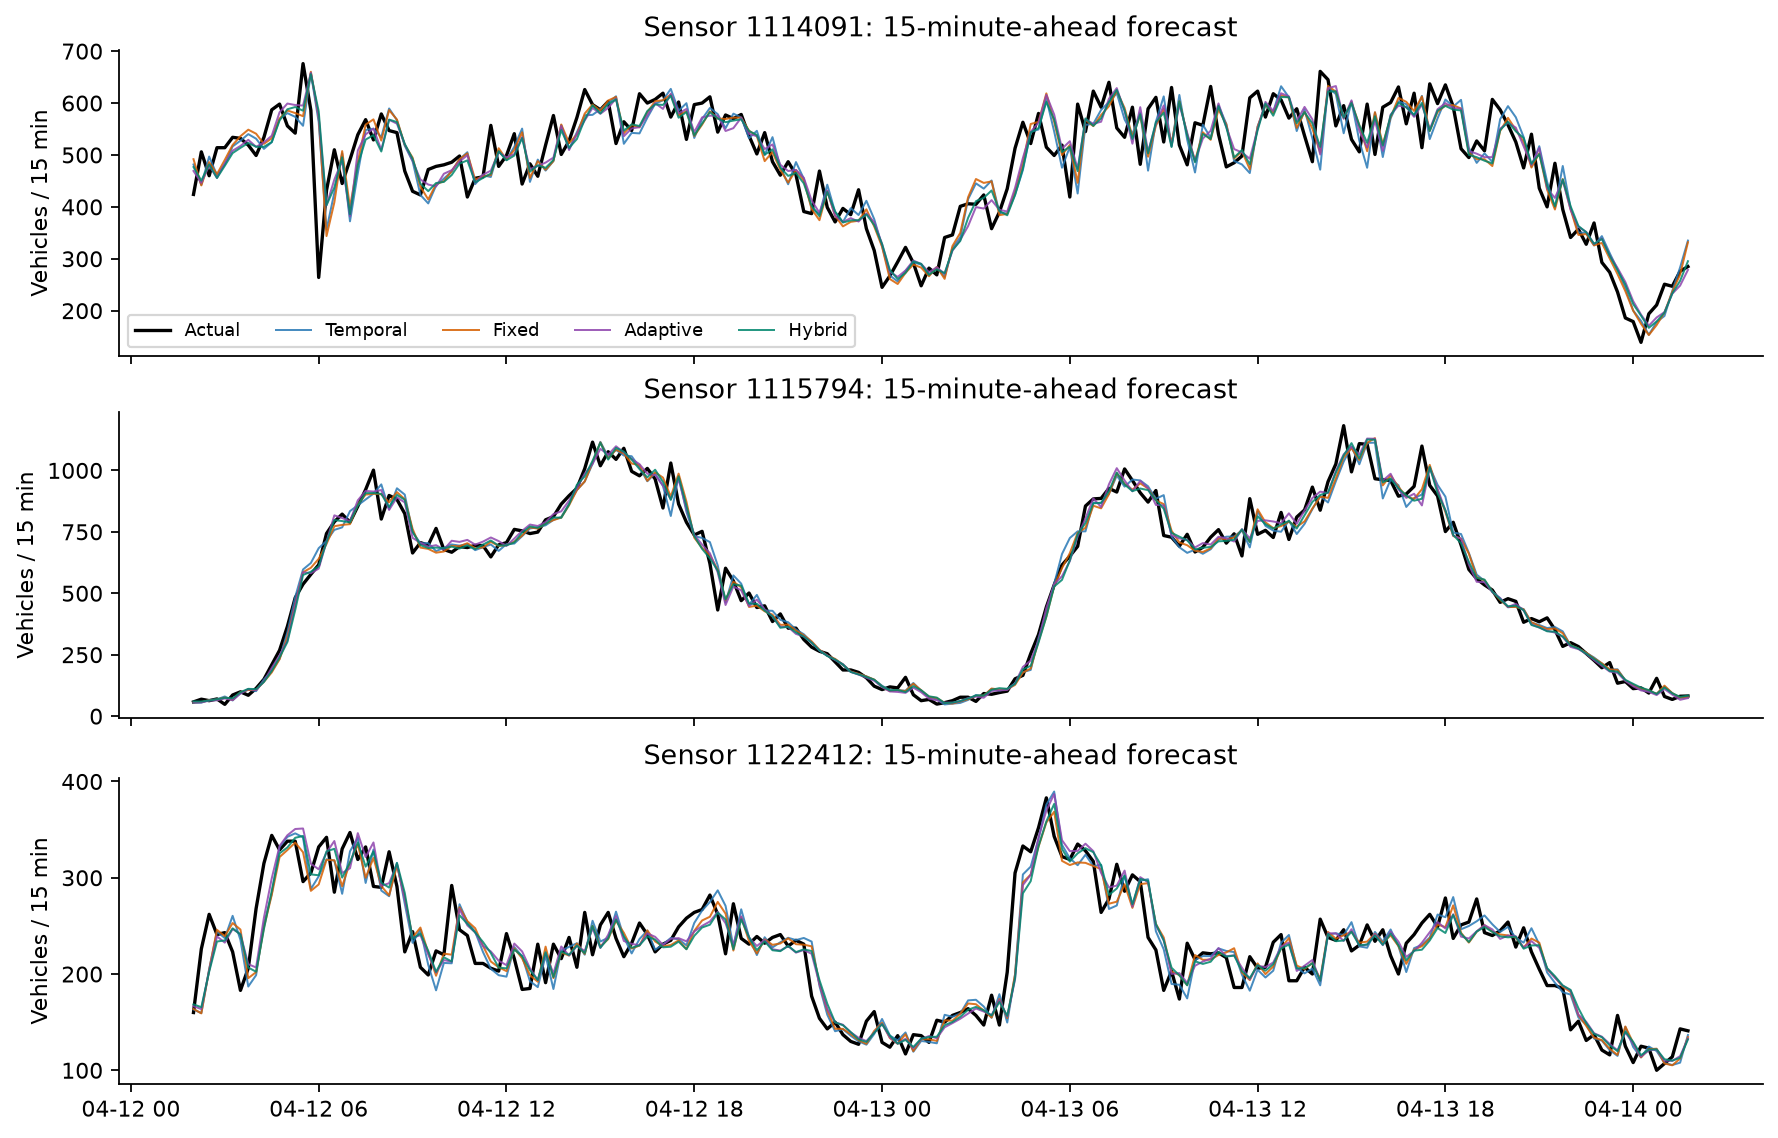
\includegraphics[width=\linewidth,height=.44\textheight,keepaspectratio]{q6_predictions.png}
\caption{Predicted and observed volume at sensors chosen by graph order (0,358,715), using input starts on 12-13 April 2021. Every line uses the same timestamps; missing observed labels are left as gaps.}
\end{figure}

\begin{table}[H]
\centering\small
\caption{Test MAE by forecasting horizon.}
\renewcommand{\arraystretch}{1.16}
\begin{tabularx}{\linewidth}{@{}>{\raggedright\arraybackslash}X>{\raggedright\arraybackslash}X>{\raggedright\arraybackslash}X>{\raggedright\arraybackslash}X>{\raggedright\arraybackslash}X@{}}
\toprule
\textbf{Model} & \textbf{15-min MAE} & \textbf{30-min MAE} & \textbf{45-min MAE} & \textbf{60-min MAE} \\
\midrule
Temporal & 43.89 & 56.50 & 67.65 & 78.96 \\
Fixed & 42.53 & 54.05 & 64.15 & 74.80 \\
Adaptive & 39.71 & 49.17 & 57.23 & 64.76 \\
Hybrid & 41.01 & 51.05 & 60.05 & 68.33 \\
\bottomrule
\end{tabularx}
\end{table}


Let \(m_{s,h,i}\) indicate an originally valid target, and let \(C=\sum_{s,h,i}m_{s,h,i}\). With predictions returned to physical units,
\begin{align}
\operatorname{MAE}&=\frac{1}{C}\sum_{s,h,i}m_{s,h,i}\left|\widehat y_{s,h,i}-y_{s,h,i}\right|,\\
\operatorname{RMSE}&=\sqrt{\frac{1}{C}\sum_{s,h,i}m_{s,h,i}\left(\widehat y_{s,h,i}-y_{s,h,i}\right)^2}.
\end{align}
The sums cover every permitted window, sensor and forecast horizon. Per-batch sums use FP32 on Arc and accumulate in CPU FP64. All models share dates, masks and normalization.


RMSE gives greater influence to large failures than MAE. Missingness may be nonrandom, so these scores characterize the observed subset of sensor-bins and cannot measure performance on unavailable ground truth. One seed and one small architecture limit any claim about the general superiority of spatial modeling.


\FloatBarrier\subsection{Learned graph structure}
For each node, select its ten strongest learned non-self edges, giving 7,160 ordered edges. This is a post-training diagnostic only. Compare exact edge overlap with the original non-self road graph and great-circle separation from sensor coordinates. Distances are geographic, not road-network path distances.


\begin{table}[H]
\centering\small
\caption{Learned top-ten non-self links and geographic reference.}
\renewcommand{\arraystretch}{1.16}
\begin{tabularx}{\linewidth}{@{}>{\raggedright\arraybackslash}p{.30\linewidth}>{\raggedright\arraybackslash}X>{\raggedright\arraybackslash}X>{\raggedright\arraybackslash}X>{\raggedright\arraybackslash}X@{}}
\toprule
\textbf{Graph / reference} & \textbf{Road overlap} & \textbf{Mean km} & \textbf{Median km} & \textbf{Within 5 km} \\
\midrule
Adaptive learned component & 4.75\% & 26.38 & 21.22 & 8.14\% \\
Hybrid learned component & 2.29\% & 29.80 & 25.40 & 4.27\% \\
Uniform non-self pair reference & 3.38\% & 27.09 & - & 5.90\% \\
\bottomrule
\end{tabularx}
\end{table}


The hybrid row in this table analyzes its learned component alone, rather than the mixed matrix that mechanically contains fixed-road edges. The uniform-pair reference describes all 716\ensuremath{\times}715 off-diagonal possibilities; it is not a separately fitted random graph. Selection ties are resolved deterministically by NumPy index sorting.


The retrained adaptive top-ten links overlap the road graph at 4.75\%, versus its density of 3.38\%. Their mean geographic separation is 26.38 km, versus 27.09 km across all non-self pairs and 2.28 km for road edges. Thus they are more local on average than uniform pairs. Geographic proximity and exact physical connectivity remain different properties.


Adaptive row entropy starts at 3.314 nats and is 3.218 at the selected checkpoint (uniform: 6.574); mean learned self-weight is 0.00500. The standard-normal initialization avoids the previous almost-flat starting graph. Entropy describes concentration, not physical correctness: top-ten membership still needs independent interpretation.


\begin{figure}[H]\centering
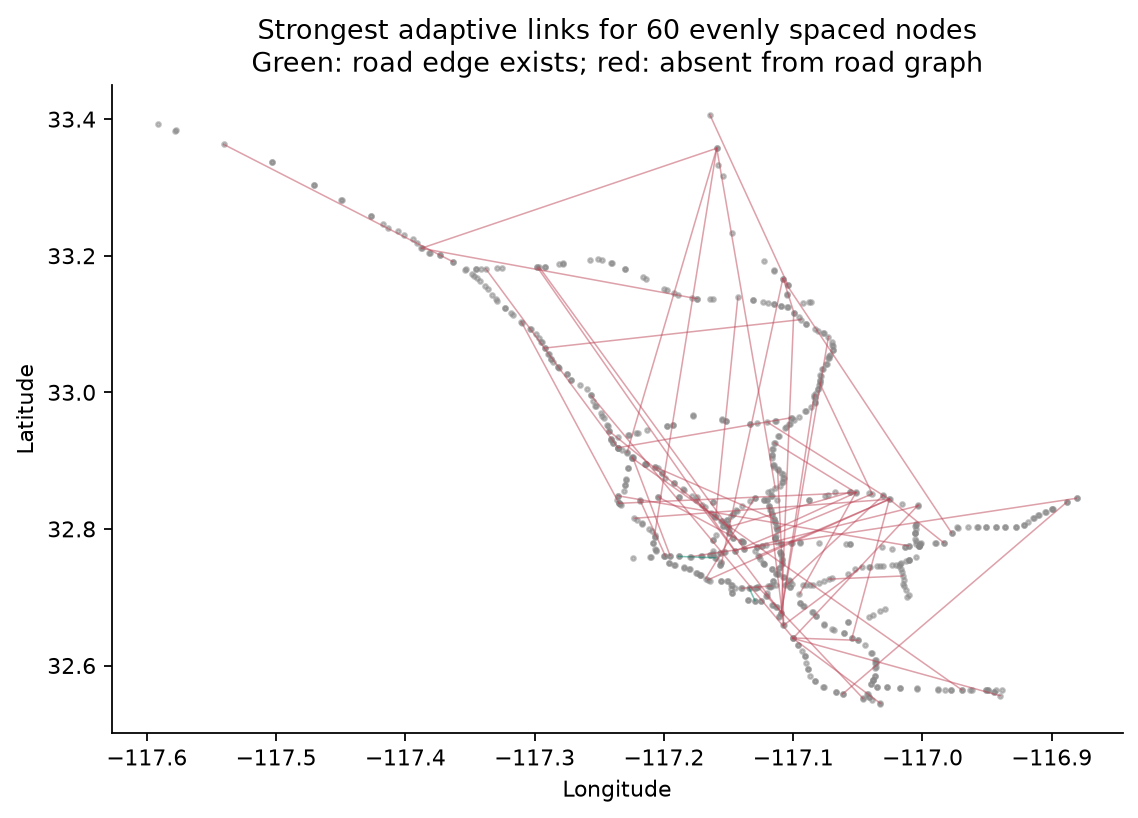
\includegraphics[width=\linewidth,height=.34\textheight,keepaspectratio]{q6_learned_map.png}
\caption{Strongest non-self adaptive link for each of 60 evenly spaced node indices, plotted at actual coordinates. Straight segments show learned associations, not road routes.}
\end{figure}

Connections absent from the road graph are possible because every pair has a trainable embedding-product logit. They can represent common commuting demand or synchronized usage patterns. They can also reflect confounding, noise or overfitting. Better held-out forecasts would support their predictive usefulness, while causal or physical meaning needs independent evidence.


\FloatBarrier\subsection{Critical discussion}
Lower forecasting error does not establish actual road connectivity: many graphs can generate similar predictions, node embeddings are not uniquely identifiable, and correlated demand can connect distant roads. A fixed graph supplies a useful structural prior and may generalize with fewer parameters. An adaptive graph can discover missing associations but may overfit or average away distinctive sensor behavior. The hybrid can balance those effects; it is not guaranteed to dominate either term.


The revised architecture retains a local path and uses per-sensor training-only scaling; it therefore avoids forcing a sensor to inherit its neighbors' raw volume level. The independent review motivated several changes together (architecture, scaling, initialization and training budget), so before/after gains cannot be attributed to one change in isolation. A static graph still misses rush-hour changes, incidents and propagation delays. Additional seeds, controlled ablations and time-dependent or delayed graph messages are useful next steps. The required 2020-2021 split includes substantial demand shift.


\section{Reproducibility and hardware execution}\label{sec:q7}\subsection{GPU training and NPU deployment}
All four networks are trained on Intel Arc through native PyTorch XPU kernels. This PyTorch installation has no Intel NPU autograd backend; OpenVINO supplies deployment inference. The NPU is selected explicitly, without AUTO or CPU fallback. Batch 16 failed NPU compilation with "Max striding levels exceeded"; static batch one succeeded. The trained learned graph is frozen only when exporting for inference.


\begin{table}[H]
\centering\small
\caption{Full-test Intel AI Boost NPU inference (static batch one).}
\renewcommand{\arraystretch}{1.16}
\begin{tabularx}{\linewidth}{@{}>{\raggedright\arraybackslash}X>{\raggedright\arraybackslash}X>{\raggedright\arraybackslash}X>{\raggedright\arraybackslash}X>{\raggedright\arraybackslash}X@{}}
\toprule
\textbf{Mode} & \textbf{NPU MAE} & \textbf{NPU RMSE} & \textbf{Full-test s} & \textbf{Median batch (ms)} \\
\midrule
Temporal & 61.75 & 97.28 & 26.4 & 0.823 \\
Fixed & 58.88 & 92.48 & 24.0 & 0.729 \\
Adaptive & 52.71 & 83.57 & 24.8 & 0.790 \\
Hybrid & 55.11 & 87.20 & 25.1 & 0.770 \\
\bottomrule
\end{tabularx}
\end{table}


{\small Every NPU run evaluates the complete test set, at batch one and device-default FP16 execution. Full-test time includes window packing, inference and metric accumulation but excludes compilation and five warmups. Batch latency times the synchronous inference call and output copy. GPU latency uses batch 16 and resident inputs, so those latency measurements are not directly comparable. FP16 can slightly change errors; exact raw values and first-batch FP32 differences are retained in results/npu\_metrics.json.}


Drivers: Intel(R) AI Boost: 32.0.100.5600; Intel(R) Arc(TM) 140T GPU (23GB): 32.0.101.9175. Python 3.12.14. Exact package versions, CPU/GPU descriptions, random seed, per-epoch histories, validity checks, graph arrays, predictions and checkpoints accompany the code.


\subsection{Reproduction}

Use an XPU-enabled PyTorch environment. Install requirements.txt without replacing the XPU wheel, then register its Jupyter kernel as ai651-xpu. Run src/download\_data.py, execute notebooks 01 through 04 in order, and run src/build\_report.py. The README includes exact commands, evaluation-only instructions and the pinned dataset provenance. Raw CA files and the large prepared cache are excluded from Git; download\_data.py recreates them.


Checks verify sensor identity/order, complete date grids, split-local windows, target masks, training-only per-sensor statistics and inverse scaling, one unit self-loop, row-stochastic graphs, nonzero embedding gradients, the independent local path and identical shared initial weights. Executed notebooks, persistence measurements and saved checkpoints make the outputs inspectable.


\FloatBarrier\appendix\section{AI Acknowledgement}
\textbf{Tool:} OpenAI Codex. Generative AI was used extensively to produce the mathematical explanations, source implementation, data pipeline, experiments, plots, notebook structure and this report. This submission should not be represented as unaided student work.


\textbf{User prompt (verbatim):}


You are an excellent standford Deep learning instructor who teaches Deel Learning for space time and graph, complete this assignment as per instructions and attached assignment document. For training and inference use intel Arc 140T gpu on this machine using pytorch optimizied libraries for intel - they are already installed and available Use Intel builtin NPU where you can for again training and inference. Upload the source code on github I have already logged in to the builtin browser https://github.com/msbasit Name: Muhammad Sami Ul Basit Roll No: 25280025.


\textbf{AI output:} the complete source in src/, four executed notebooks, measured experiment artifacts and checkpoints, seven figures, README reproduction instructions, and this PDF. The generated code was executed on the stated hardware; tabulated results come from saved measurements rather than invented examples.


\textbf{Initial implementation and verification:} Codex selected the installed Intel XPU environment, used a pinned dataset mirror after Kaggle API failures, accumulated metric totals in CPU FP64 after XPU FP32 reductions, and reduced NPU batch size to one after a compiler failure. Automated checks and PDF rendering support the execution record. The subsequent model corrections and report revisions were directed by the independent human review described below.


\textbf{Style-revision prompt:} "I dont really like the style of the report. I like conventional report style with Latex based equations and expressions"


\textbf{Earlier style revision:} on 22 November 2026, the report was retypeset with native LaTeX equations, serif typography, numbered sections, conventional tables, figure captions and references. The editable TeX source is included. That formatting-only revision retained the then-current results; the subsequent review-driven reruns are described below.


\textbf{Human contribution and independent review:} I independently reviewed the earlier solution against the assignment. I checked the Q1-Q2 derivations and data/split conventions, identified weaknesses in the model design, initialization and training budget, and supplied specific corrections and report revisions. I directed these changes and reviewed the implementation choices. Codex assisted with implementation, retraining, automated checks and artifact regeneration. This work therefore includes substantive human review and intervention alongside AI assistance.


\textbf{Correction request (summary):} following my independent review, I asked Codex to review and fix the documented problems, and to discuss any points of disagreement with me first. The private review notes are excluded from the report, public repository and submission archive.


\textbf{Review-driven edits:} added a local feature path, standard-normal 10-dimensional node embeddings, per-sensor training-only normalization and inverse scaling, a single-self-loop convention, a 40-epoch maximum with patience 5, persistence checks, and corrected wording. A final graph diagnostic identified embedding collapse under coupled weight decay; excluding the embeddings from decay and rerunning adaptive/hybrid corrected that problem. All four models were retrained and re-evaluated on GPU; NPU inference, plots, graph diagnostics, conclusions, source and submission artifacts were regenerated. These are AI-agent implementation edits following my independent review; the new numerical outputs are supported by saved execution records.


LargeST is released under CC BY-NC 4.0 \cite{largest-repo}. Raw dataset files are not redistributed in this repository. The small derived SD adjacency and sensor metadata retain their source attribution and noncommercial data license. Source code is provided for academic reproducibility.


\FloatBarrier
\begingroup\small
\begin{thebibliography}{9}\setlength{\itemsep}{2pt}\setlength{\parskip}{0pt}
\bibitem{largest-repo} X. Liu et al. \emph{LargeST: official repository and preprocessing notebooks}. \url{https://github.com/liuxu77/LargeST}.
\bibitem{mirror} \emph{Public LargeST raw-data mirror}. Pinned revision and SHA-256 values appear in \texttt{results/download\_provenance.json}. \url{https://huggingface.co/datasets/ttydsc30/TrafficForecast-LargeST-Project-Dataset}.
\bibitem{pems} Caltrans. \emph{PeMS Traffic Data Downloads: five-minute station total flow}. \url{https://pems.dot.ca.gov/?dnode=Clearinghouse}.
\bibitem{largest-paper} X. Liu et al. ``LargeST: A Benchmark Dataset for Large-Scale Traffic Forecasting.'' \emph{NeurIPS Datasets and Benchmarks}, 2023. \url{https://arxiv.org/abs/2306.08259}.
\bibitem{pytorch} PyTorch. \emph{Getting Started on Intel GPU}. \url{https://docs.pytorch.org/docs/stable/notes/get_start_xpu.html}.
\bibitem{openvino} Intel. \emph{OpenVINO: NPU Device}. \url{https://docs.openvino.ai/2025/openvino-workflow/running-inference/inference-devices-and-modes/npu-device.html}.
\end{thebibliography}
\endgroup
\end{document}
